\chapter{Centroidal estimation}
\label{chp:centroidal_estimation}
\minitoc
\bigskip


In this chapter, we propose a tightly-coupled estimator of the base and centroidal states that fuses IMU, kinematics, centroidal kinematics, 
and force-torque measurements. This work was first presented in our published paper \cite{fourmy2021contact}.

\section{Introduction}

As mentioned in the literature review, centroidal states are key to the control of legged robots. Indeed, they provide rich information about the general
behavior of the system and can be used to check for the stability of the system. The centroidal state estimation literature is rich, especially for humanoid
robots (see \secRef{sec:centroidal_est_lit}). To our knowledge, all of the centroidal estimators proposed in the literature can be classified as loosely-coupled estimators 
(following the terminology introduced in \secRef{sec:proprio_filters}): they rely on prior knowledge of a base state. For instance, Piperakis \cite{piperakis2018nonlinear} 
describes the whole pipeline: first, an inertial-kinematics EKF estimates the base state, then an EKF uses this fixed base state to obtain centroidal states. 
Since the factor graph optimization framework that we use theoretically reaches its full potential when the maximum number of cross-correlation
are considered, we did not find this solution satisfactory. Here, we rather propose a tightly-coupled estimator that jointly estimates
base and centroidal states using IMU, kinematics, and force measurements.



To the best of our knowledge, this is the first time an estimator tightly couples forces, IMU, and proprioception to estimate both base and centroidal
quantities. This estimator finds its roots in visual-inertial SLAM as described in the previous chapter,
and in the observability studies of centroidal quantities, already discussed in \secRef{sec:centroidal_dynamics}. We then skip here a discussion of related
works which has been sufficiently covered, to directly describe the underlying factor before exhibiting the experimental results.


% We present results of the application of the estimator on a dataset taken at LAAS-CNRS on the open-source robot Solo-12 \cite{grimminger2020open}:
% \textit{sinXYZ} corresponds to a trajectory where the robot moves by following a sine wave reference with the feet fixed in place. 
% This movement and another one are displayed in the companion video \url{https://peertube.laas.fr/videos/watch/16822d27-3557-4e35-9a0d-ce5b0aea4c27}.

% We use the state estimation framework WOLF developed at IRI-Barcelona, which relies on Google Ceres \cite{ceres-solver} as the graph solver. 
% The robot kinematics and dynamics computations are handled by the Pinocchio library \cite{carpentier2019pinocchio}. For all runs, \keyframes\ were created 
% at 4Hz for a fair comparison.



\section{Problem statement}

We define here an estimator capable of observing both base states (position, orientation, velocity) and centroidal states (CoM, CoM velocity, angular momentum) from proprioception
only. We assume that the following measurements are available on the robot: IMU data, kinematics (leg odometry), centroidal kinematics, and force-torque sensors. 
Since the IMU measurements \eqRef{eq:imu_meas_model} and CoM local position from the kinematics \eqref{eq:com_kine_meas} are biased, we also need to integrate them to the estimated
variables.

Bloesch \cite{bloesch2013state} showed that the base states of legged robots and IMU biases are observable using a tightly-coupled estimator based on IMU and kinematics measurements.
On the other end, Rotella \cite{rotella2015humanoid} showed that the centroidal state of a robot and a bias on the centroidal kinematics can be obtained by fusing 
force-torque sensor measurements with centroidal kinematics, based on prior knowledge of the base states. We join the two problems into a single state estimation problem, 
represented by the factor graph of \figRef{fig:centroidal_factor_graph}.  

\begin{figure}[t]
    \centering
    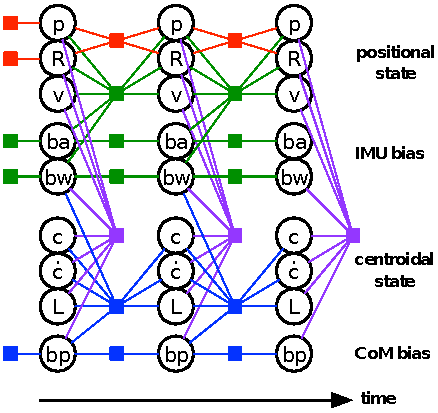
\includegraphics[width=0.6\textwidth]{figures/centroidal/centroidal_factor_graph.pdf}
    \caption{Factor graph representation of the tightly-coupled base-centroidal state estimation problem.
             Each round node corresponds to an estimated state variable. Each square corresponds to a factor, that is a measurement residual.
             The colors of the residuals are as follows. \textbf{Red}: leg odometry (\secRef{sec:leg_odometry}), \textbf{green}: IMU pre-integration and IMU bias drift 
             (\secRef{sec:preint_residual}), \textbf{purple}: centroidal kinematics (\secRef{sec:centroidal_kinematics}), \textbf{blue}: force-torque pre-integration and
             centroidal kinematics bias drift (\secRef{sec:force_torque_preint}).
             }
    \label{fig:centroidal_factor_graph}
\end{figure}

In this estimator, we have two motion sensors, IMU and force-torque, whose measurements we pre-integrate as explained in \secRef{sec:imu_preint_composite} and
\secRef{sec:force_torque_preint} respectively. Base states and centroidal states are tightly constrained by the centroidal kinematics factor, which relates almost all 
estimation variables at a given \keyframes.

\section{Experimental setup}
\label{eq:expe_setup_centroid}

This estimator is implemented in WOLF \cite{sola2021wolf}, with necessary kinematics and dynamics quantities computing
with Pinocchio software \cite{carpentier2019pinocchio}, and is experimentally validated on the Solo-12 quadruped robot. 

As is often the case with quadruped robots, Solo-12 is not equipped with three-axis force sensors at its feet. 
Yet, in order to validate the present method, it is possible to reconstruct the contact forces based on the robot dynamics 
equation \eqref{eq:wbdyn}. Knowing the robot configuration and derivatives $\q,\vq,\dvq$, and joint torques $\bm\tau$ (from motor currents), 
recovering forces from this equation results in solving an over-determined linear system. Some of these quantities are hard to obtain directly 
since they depend on the state being estimated (\eg base orientation) or on numerical differentiation ($\ddqa$). For these reasons, we pre-calculated 
these forces by benefiting from an internal filter of the 3DM-CX5-25 IMU for the base orientation, centered window differentiation of encoder speed 
measurements for the articulation acceleration $\ddqa$, and neglecting the influence of linear velocity. Fig. \figRef{fig:force_est} shows an example of 
the force reconstruction of one leg using the robot proprioceptive sensors.
%
\begin{figure}
    \centering
    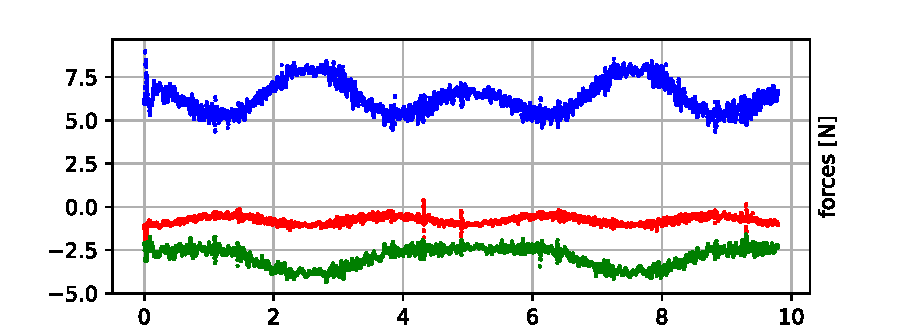
\includegraphics[width=0.9\columnwidth]{figures/centroidal/forces_solo_1leg.pdf}
    \caption{Force estimation on X-Y-Z axis (r-g-b) of one Solo-12 leg expressed in world frame using proprioceptive sensors during the \textit{sinXYZ} trajectory}
    \label{fig:force_est}
\end{figure}

This movement and another one are displayed in the video \url{https://peertube.laas.fr/videos/watch/16822d27-3557-4e35-9a0d-ce5b0aea4c27}.
The configuration trajectories were obtained using task space inverse dynamics \cite{adelprete:jnrh:2016} and applied to the robot with joint-level admittance control.


\section{Results}

\subsection{Base estimation through inertial kinematic fusion}
First, to validate the use of our kinematic factor, we include uniquely the IMU and leg-odometry factors to obtain an Inertial Kinematics estimator which 
conceptually includes the same information as estimators such as \cite{bloesch2013state}. In \figRef{fig:PosiIK4}, we compare our state estimation 
at 1kHz with motion capture (Mo-Cap) up-sampled from 200Hz to 1kHz.
Velocity in the base frame is also shown in \figRef{fig:VelIK4}.

\begin{figure}[h]
    \centering
    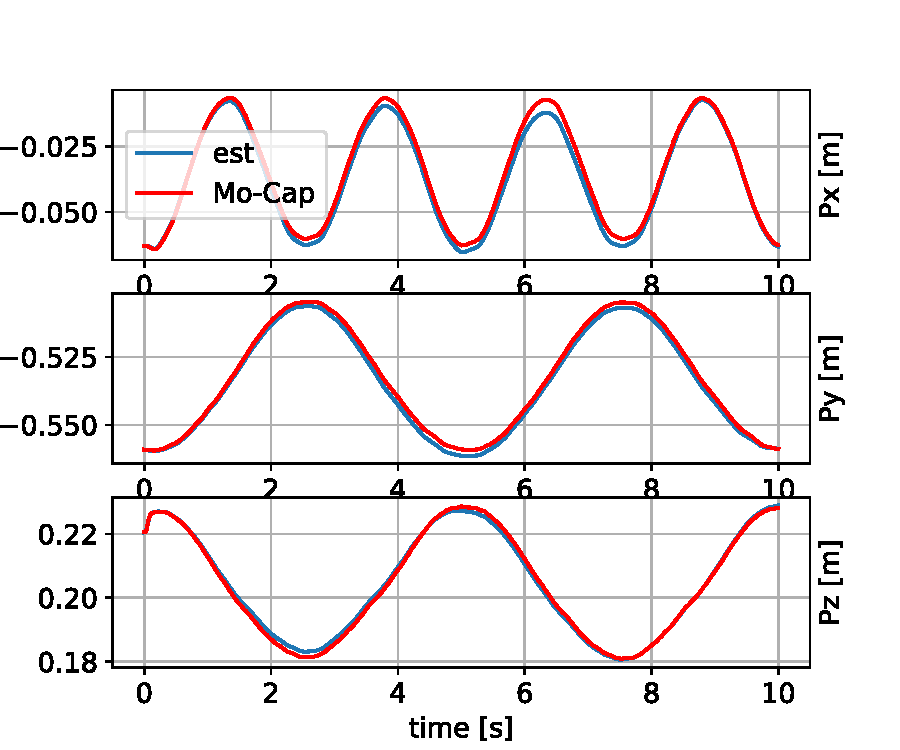
\includegraphics[width=0.6\textwidth]{figures/centroidal/base_position_IK4.pdf}
    \caption{\textit{sinXYZ} trajectory base position from the IMU+Kinematics (IK) estimator (blue) vs Mo-Cap (red)}
    \label{fig:PosiIK4}
\end{figure}

\begin{figure}[h]
    \centering
    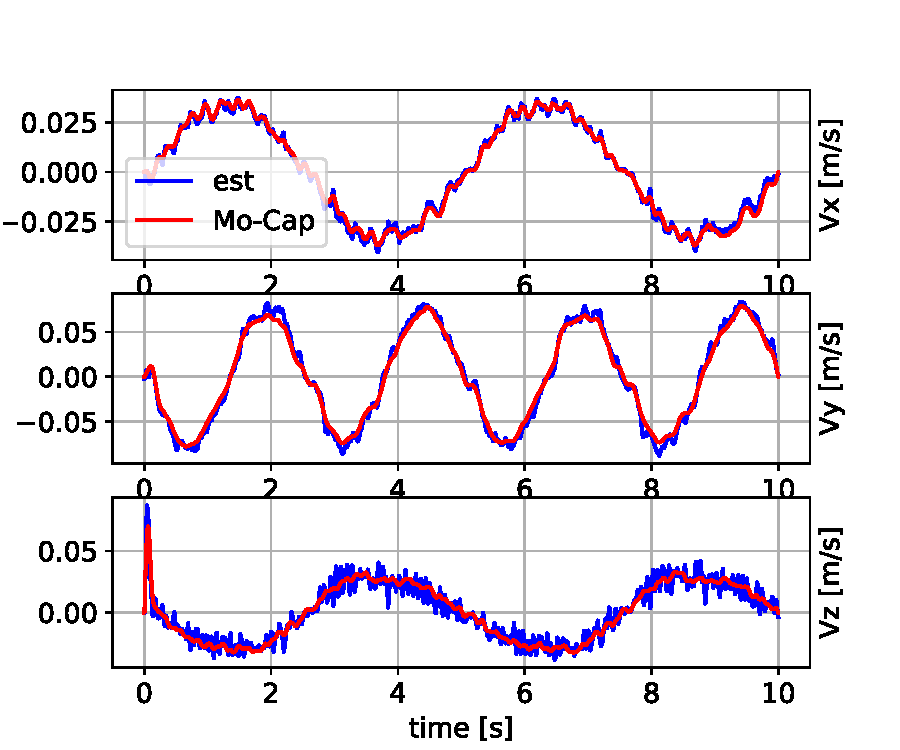
\includegraphics[width=0.6\textwidth]{figures/centroidal/base_velocity_base_frame_IK4.pdf}
    \caption{\textit{sinXYZ} trajectory base velocity in base frame from the IMU+kinematics estimator (blue) vs Mo-Cap (red)}
    \label{fig:VelIK4}
\end{figure}

Artificially removing contact factors (considering only 1, 2, or 3 feet in contact) can help us gain confidence in the use of this kinematic factor 
in situations where we rarely have all feet in contact, like for example with trotting gaits. In \figRef{fig:ErrIKn}, we can see that only considering 
1 foot in contact during the whole trajectory results in a drifting position, but as soon as 2 or more feet are in contact, the system is constrained enough 
for the drift to remain below around 5mm on all axes. 
%
\begin{figure}[h]
    \centering
    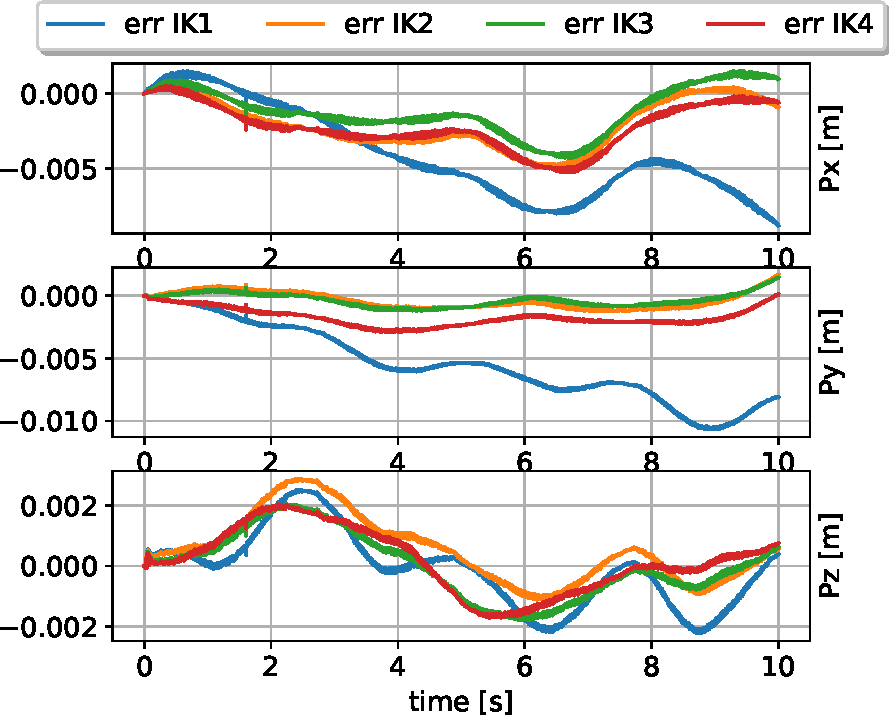
\includegraphics[width=0.6\textwidth]{figures/centroidal/base_position_err_IKn.pdf}
    \caption{\textit{sinXYZ} trajectory base position error with different numbers of feet used for the leg-odometry factors: 
    1 (blue), 2 (orange), 3 (green), 4 (red) from the IMU+kinematics estimator}
    \label{fig:ErrIKn}
\end{figure}
%

\subsection{Centroidal estimation}

Now, on the same trajectory, we deploy the full estimator with all factors described in the factor graph in \figRef{fig:centroidal_factor_graph} to jointly 
estimate the base and centroidal quantities. A ground truth on the centroidal quantities is difficult to obtain since no direct 
sensor can provide us with this information contrary to the base state. 
We can however validate our method by comparing it to a two-step procedure: first, estimate the base state with a state Kalman filter as 
implemented in \cite{bledt2018cheetah}, then compute the centroidal quantities directly from the robot kinematic model. 
The full estimator should be able to infer a bias on the $\posim{B}{C}$ measure so we artificially add a constant disturbance 
in the robot dynamic model on the lever of the base link of [0.03, 0.06, 0.04]\,cm, which then corresponds to a CoM bias of 
[-0.0197, -0.0394,  0.0263] cm. \figRef{fig:bias_est} shows that the bias estimated with our method closely matches the introduced bias. 
\figRef{fig:comparison_KF_wolf} shows a comparison between the base and CoM reconstruction with our method and with the two-step base Kalman filter 
with geometric CoM. Note that the base-CoM difference on the z-axis reflects the fact that the limbs of the robot naturally lower its CoM. 
The estimated CoM velocity closely follows the velocity of the base as shown in \figRef{fig:com_base_vel}.


\begin{figure}[h]
    \centering
    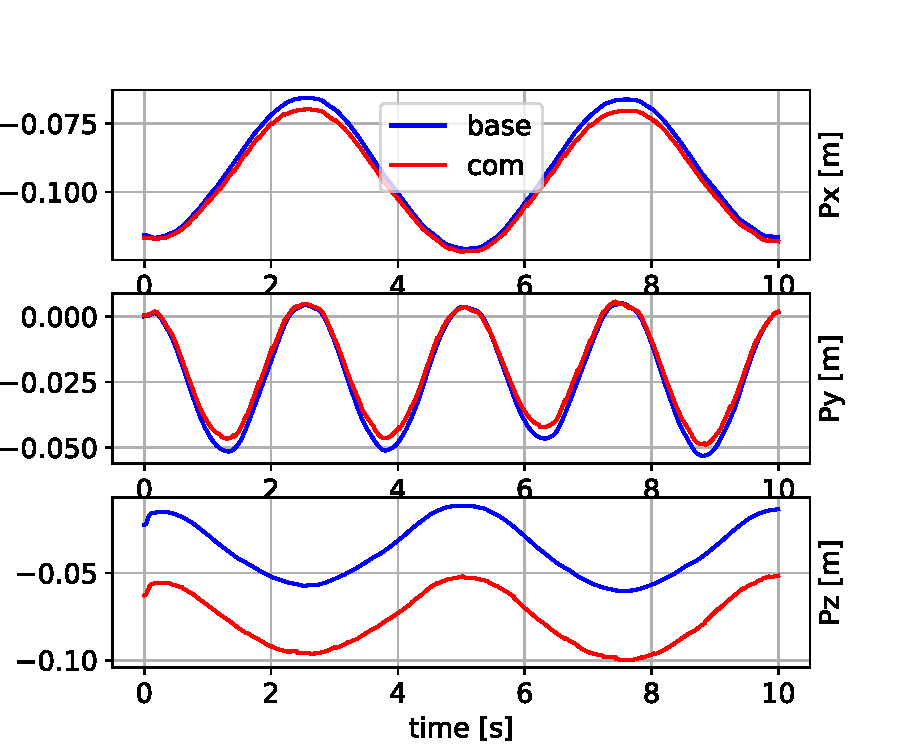
\includegraphics[width=0.6\textwidth]{figures/centroidal/com_position_povcdl_sin.pdf}
    \caption{Base position (blue) vs CoM (red) from the full estimator}
    \label{default}
\end{figure}

\begin{figure}[h]
    \centering
    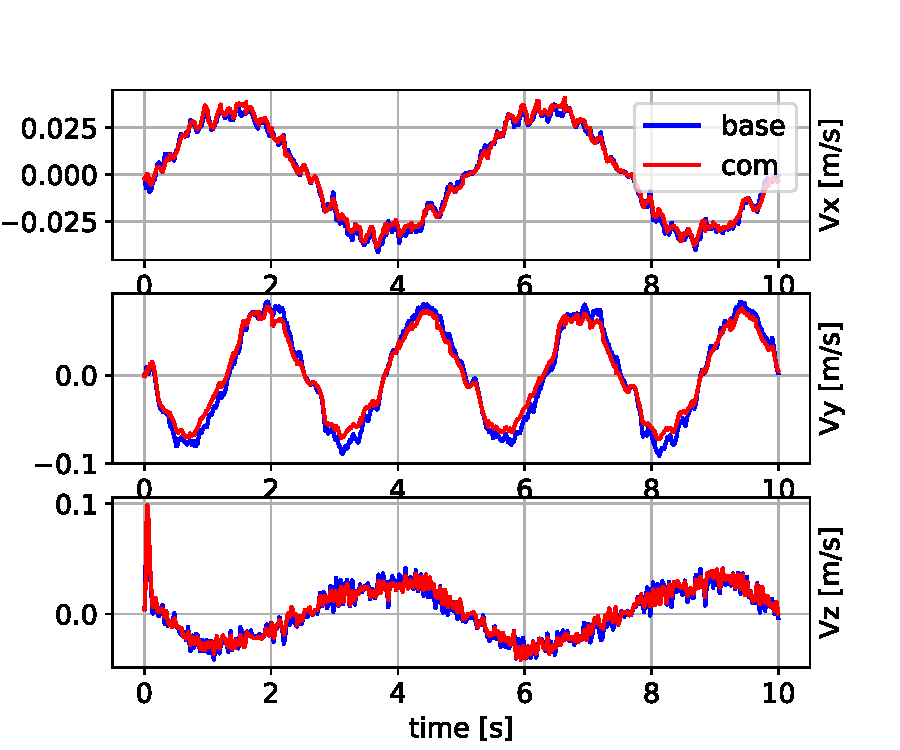
\includegraphics[width=0.6\textwidth]{figures/centroidal/com_velocity_povcdl_sin.pdf}
    \caption{Base (blue) vs CoM (red) velocities   from the full estimator}
    \label{fig:com_base_vel}
\end{figure}


\begin{figure}[h]
    \centering
    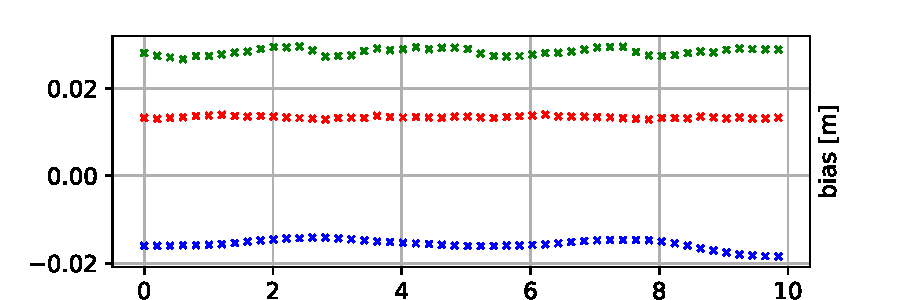
\includegraphics[width=0.6\textwidth]{figures/centroidal/com_bias_est.pdf}
    \caption{Estimation of bias on CoM measurement from the full estimator along x-y-z axis ( red-green-blue) in base frame}
    \label{fig:bias_est}
\end{figure}

\begin{figure}[t]
    \centering
    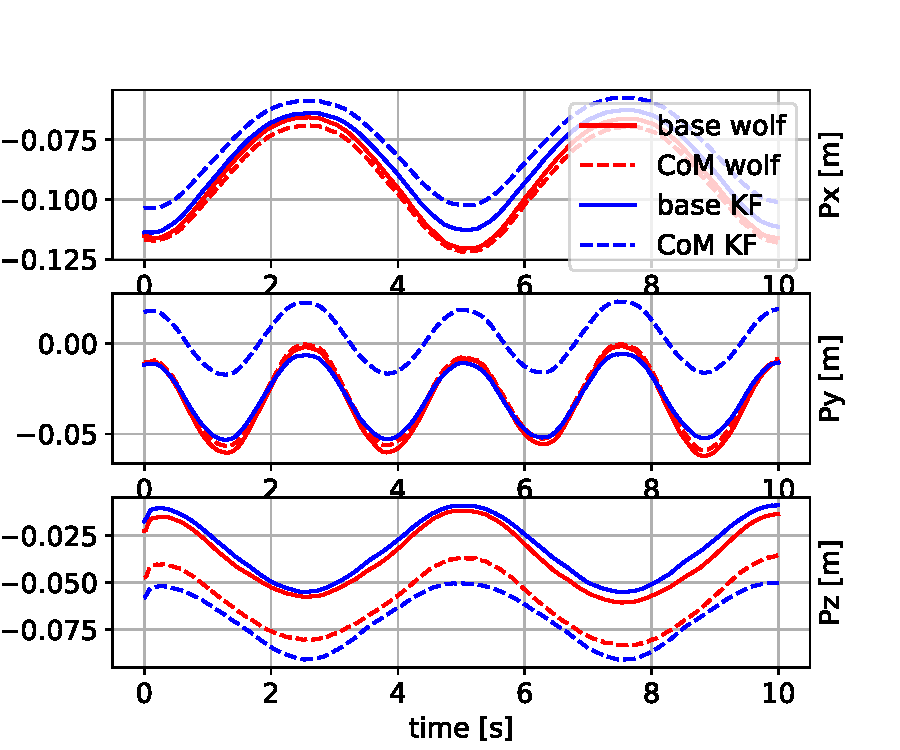
\includegraphics[width=0.6\textwidth]{figures/centroidal/base_com_position_wolf_vs_KF.pdf}
    \caption{Comparison of the estimates between decoupled the Kalman filter base estimator and geometric CoM reconstruction (blue) and 
    the tightly-coupled estimator presented in this paper (red) on the \textit{sinXYZ} trajectory with artificial base link CoM bias.}
    \label{fig:comparison_KF_wolf}
\end{figure}


\section{Discussion}

On the theoretical side, the correlation of the IMU and forces pre-integration models (due to the common gyroscope data integration) might also be investigated. 
One of the hypotheses involved in factor graph MAP estimation is the conditional independence of measurement data (see \eqRef{eq:factorized_likelihood} in \secRef{sec:MAP} for more details).
Using the same measurements for both factors violates this assumption. Our model is not an exception in MAP estimation: for example, \cite{wisth2019robust} uses 
integrates the velocity output of an inertial-kinematic filter to obtain an odometry factor, while using IMU data in an IMU-preintegration factor. In our case,
a solution would be to derive an algorithm pre-integrating IMU and force data at the same time. This choice would be at the cost of the modularity of the 
use of two separate factors.  

While the results correspond to the expectation, several aspects of the experimental protocol would benefit from 
improvements in the future. First, the experimental platform we used is not the most appropriate to implement this type of estimator.
Indeed, Solo-12 does not have force-sensors at the feet, which required the force estimation procedure described in \secRef{eq:expe_setup_centroid}.
The inconvenience of this method is two-fold. Firstly, the estimated forces make heavy use of the IMU acceleration measurements which makes the forces pre-integration
correlated with IMU pre-integration. Secondly, the force estimation gave us good performances only for rather slow trajectories, which prevented their use for walking
trajectories for instance. We could have turned our interest to our humanoid robot Talos (see \figRef{fig:robots}) which features force-torque sensors at its feet.
However, at the time, Solo-12 was still a safer choice for several issues with Talos, that have since been partially addressed (kinematic calibration, higher flexibility of the 
structure, biased feet force sensors).



Nevertheless, Solo-12 allowed us to easily generate datasets based on simple quasi-static trajectories. We since recorded more datasets with walking trajectories
based on the walking controller \cite{leziart2021implementation}, including the robot proprioceptive measurements as well as images from an onboard camera (See \chpRef{chp:dataset} for more details). Evaluation
of our inertial-kinematic estimator on these new trajectories is ongoing (see \chpRef{chp:dataset}).




\section{Conclusion}

To the best of our knowledge, the work presented in this chapter corresponds to the first demonstration of the feasibility of tightly coupling the estimation
of both the robot basis and its centroidal state. Beyond the practical limitations of our experimental setup, it opens the
road to more ambitious filters able to provide a consistent by design estimation of the quantities needed for balance
control and navigation, which we believe to be essential for reaching safe locomotion on 3d terrains. Our main effort
is now to extend this work to also integrate advanced exteroceptive measurements able to provide meaningful information
about the surrounding environment, as will be explained in the next chapter. We then see exciting perspectives in extending
this estimator to multiple other information sources on the robot's whole body, to tightly couple the estimation of a more
complete state.

